\chapter{Specyfikacja wewnętrzna}
\label{ch:05}

\section{Architektura systemu}

\note{W tej części pracy należy opisać, jakie komponenty składają się na system. Należy zaznaczyć, jakie są relacje między nimi. Można również opisać, jakie wzorce projektowe zostały zastosowane. Głównie chodzi o to, aby czytelnik mógł zrozumieć, jak działa system.}

Kompletny system składa się z czterech głównych komponentów, które komunikują się ze sobą w celu zapewnienia pełnej funkcjonalności. Poniżej zostały przedstawione opisy każdego z nich.

\subsection{Frontend}

Głównym interfejsem użytkownika jest aplikacja webowa stworzona przy użyciu frameworka \texttt{Vue.js}. Zapewnia użytkownikowi dostęp do większości funkcji systemu, a w zależności od roli użytkownika, pozwala na wykonanie innych czynności. Aplikacja została zaprojektowana w taki sposób, aby była przejrzysta i intuicyjna w obsłudze. Dzięki temu, użytkownik może szybko i sprawnie wykonywać swoje codzienne obowiązki. Odrębne od siebie panele zostały umieszczone w kartach pojawiających się na widoku, dzięki czemu użytkownik wie dokładnie w którym miejscu aplikacji się znajduje i jakie ma możliwości.

\subsection{Backend}

Serwer aplikacyjny został stworzony przy użyciu frameworka \texttt{Spring Boot}. Zapewnia on komunikację między bazą danych, a pozostałymi komponentami systemu. Jest odpowiedzialny za przetwarzanie żądań klienckich oraz zwracanie odpowiedzi w postaci danych, w formacie \texttt{JSON}. Serwer aplikacyjny jest również odpowiedzialny za autoryzację i autentykację użytkowników oraz zarządzanie sesjami. Użytkownicy nie mają bezpośredniego dostępu do serwera.

\subsection{Aplikacja mobilna}

Głównym zadaniem aplikacji mobilnej jest możliwość dodawania kart dostępowych dla poszczególnych użytkowników. Odbywa się to poprzez przyłożenie tagu NFC (ang. \english{Near Field Communication}) do telefonu z zainstalowaną aplikacją, a następnie przypisanie go do konkretnego użytkownika. Szczegółowy opis tego procesu został opisany w rozdziale \ref{sec:addNfc}.

\subsection{Układ mikroprocesorowy}

Układ mikroprocesorowy jest odpowiedzialny za odczytywanie tagów NFC oraz przesyłanie informacji do serwera aplikacyjnego. Następnie serwer zwraca informację o przyznaniu dostępu do systemu. Układ mikroprocesorowy jest zasilany z wbudowanego portu Micro USB, co umożliwia bardzo proste podłączenie go do źródła zasilania. Dokumentacja techniczna mikrokontrolera \cite{bib:picoWdatasheet} precyzuje również podłączenie innego źródła zasilania bez użycia wbudowanego portu.


\section{Modele i struktury danych}

\note{W tej części pracy należy opisać, jakie modele danych zostały zastosowane w systemie. Należy zaznaczyć, jakie są relacje między nimi.}

\subsection{Model użytkownika}

\section{Struktura bazy danych}

\note{W tej części pracy należy opisać, jakie tabele i relacje między nimi występują w bazie danych. Można dodać diagramy ERD.}

\subsection{Logowanie}

\note{Tutaj można dodać diagramy czynności i sekwencji.}

\section{Algorytmy}

\subsection{Rejestracja}

\subsection{Logowanie}

\begin{figure}[H]
    \centering
    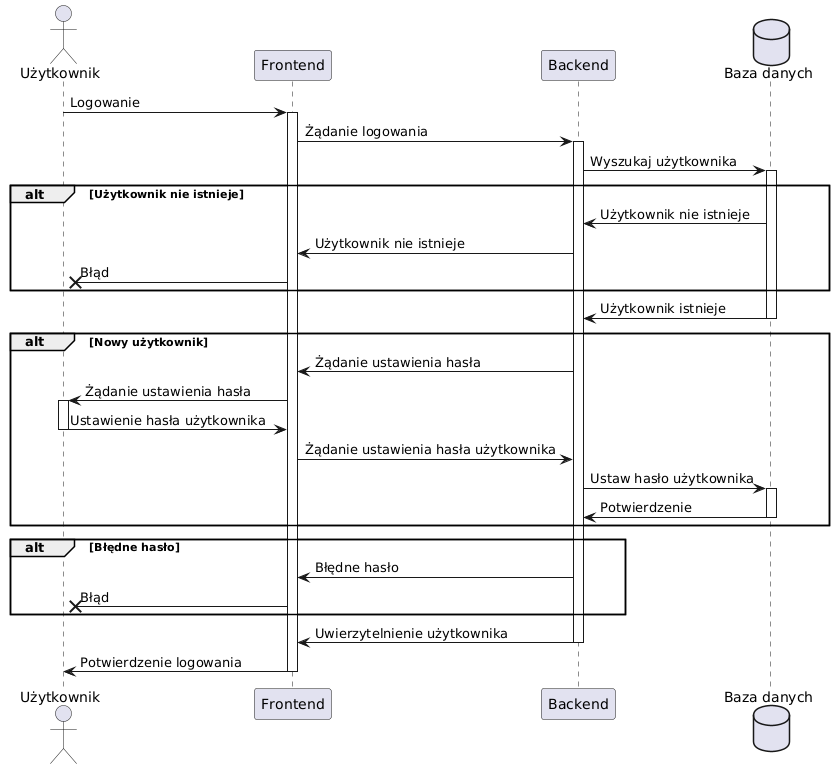
\includegraphics[width=\textwidth]{graf/loginSequence.png}
    \caption{Diagram czynności logowania}
    \label{fig:login}
\end{figure}
% //www.pantum.com/plantuml/png/VP8nRiCm34LtdKB8dWju288CdOgYIz2PigX6iIC5jbJN7WFq43rBEzRtAeceK6pKcJpyh__9Hs_R04s8frf06NmZz-Dt7ohVELj9QAMBuaowBUqPN90FZNS1dMR9u4JQGLabHQ7G4411YtArWm6a1jUNXnMBMWaXN9Jh3IN8GZxwLz-1iyW3s3S8oCa6rnl5ylZryw5PbdKoGZPIaK9EqegiBtqxn0gECkOTifcBeGwJ1JdMje4-HnfPSHANBdfIcxdhCUnv9t9aseqN6byG5uhdZMOFSpdEvtpoNN-xYL24n4oHH3fUPv6Oo0EqumK4StFnhYaZuUkwoAd5_i-4oJI5gF7cJJfEiLmnUysJQqMRi-tgy8j7Ig0A-Um3PJPweDmv80RAa9ZlftQOGZEZkM3mdvja-vwRXZvWxQuGbhPNwRuSDHin_w2t3moABLN5K_qB

\subsection{Harmonogramowanie}

\subsection{Przypisanie nowej karty dostępowej}

\section{Użyte biblioteki i frameworki}

\note{Ta część może się znaleźć przy przeglądzie technologii.}